%%
%%       --- a chapter ---
%%
%% A chapter

\chapter[Stellar Masses and Completeness Simulations]{Estimating Stellar Masses} 
\label{ch:chapter1_label}

\section[Sec]{Section}
\label{sec:section1_label}

\section{Mass Fitting}\label{sec:masses}
Stellar masses were estimated for our samples using a custom template fitting code with SEDs derived from the synthetic stellar population models of \citet{Bruzual:2003ckb} (BC03 hereafter). Due to the relatively young ages of the stellar populations (as constrained by the age of the Universe at the redshifts involved), the effects of thermally-pulsating asymptotic giant branch stars (TP-AGB) on resulting SEDs are minimal, e.g. \citet{2009ApJ...697.1493S}. As such, we chose not to use the updated SSP models which incorporate these effects. The use of Charlot \& Bruzual (2007) or \citet{Maraston:2005er} in place of BC03 should have no result on the conclusions found in this work.

Based on the method used in \citet{Hartley:2013cn} and \citet{Mortlock:2013dg}, our SED fitting code has been amended and expanded to incorporate the measurement of additional parameters described below and the inclusion of nebular emission.

\subsection{Model SEDs}\label{subsec:seds}
First, model SEDs are generated from the single stellar populations of Bruzual \& Charlot for a range of population ages, metallicities and star-formation histories (SFHs).  Each star-formation history is normalised such that at the desired model age, the total integrated SFR equals 1 M$_{\odot}$. At this stage, nebular emission lines are added to the pure stellar component following the method outlined in Section~\ref{subsection:nebular}. Internal dust extinction is applied following the extinction law of \citet{2000ApJ...533..682C} for the desired range of extinction magnitude $A_{V}$. 

When applying dust extinction to the nebular emission, we assume the differential dust extinction between stellar and nebular emissions to be fixed as $E(B-V)_{stellar} = E(B-V)_{nebular}$, in contrast to the ratio of $E(B-V)_{stellar} = 0.44 E(B-V)_{nebular}$ derived by \citet{2000ApJ...533..682C}. This choice was motivated by the conflicting evidence for the relative extinction of the two sources at $z \sim 2$ \citep{Erb:2006ke,ForsterSchreiber:2009hm} and that in the context of these models specifically, the assumed differential extinction ratio and escape fraction are degenerate.

The absolute magnitude at 1500 \AA ~(M$_{1500}$) is measured for each template by integrating the flux within a 100 \AA-wide flat bandpass centered on 1500 \AA. Similarly, the UV-continuum slope $\beta$ is calculated by fitting a simple power-law to the integrated template fluxes in the windows described in \citet{1994ApJ...429..582C}. The accuracy of this method in calculating $\beta$ is explored in \citet{Finkelstein:2012hr} and \citet{2013MNRAS.429.2456R}.

Next, each model SED is redshifted in the range $0 \le z < 9$ in steps of $\Delta z = 0.02$, and attenuation by intergalactic neutral hydrogen is applied following the prescription of \cite{1995ApJ...441...18M}. The resulting grid of SEDs is then integrated through the response filter for each of the observed bands. 

\subsection{Nebular Emission}\label{subsection:nebular}
Nebular emission lines and continuum are added to the templates following a method similar to previous high-redshift fitting methods, e.g.  \citet{Ono:2010ed,2010A&A...515A..73S,2011MNRAS.418.2074M}, Salmon et al. \emph{in prep}. Line strength ratios relative to H$\beta$ for the major Balmer, Paschen and Brackett recombination lines are taken from \cite{Osterbrock:2006ul}, with the total H$\beta$ line luminosity (in erg s$^{-1}$) given by
\begin{equation}
L(H\beta) = 4.78 \times10^{-13} (1-f_{esc}) N_{LyC}
\end{equation}
from \citet{1995A&A...303...41K}, where $f_{esc}$ is the continuum escape fraction and the number of Lyman continuum photons N$_{LyC}$ is calculated from each template. The strength of the nebular emission is therefore directly proportional to the number of ionizing photons (Lyman continuum) in the HII region. Since the Lyman continuum emission is dominated by young massive stars, the relative contribution of nebular emission to the total SED is highly dependent on the age of the stellar population and the amount of recent star-formation.  
 
Line ratios for the common metal lines relative to H$\beta$ were taken from the empirical measurements of \cite{Anders:2003ci} for each of the input template metallicities, assuming gas metallicity is equal to the stellar metallicity.
Similarly, the nebular continuum emission luminosity is given by
\begin{equation}
\label{eq:continuum}
L_{\nu} = \frac{\gamma^{(total)}_{\nu}} {\alpha_{B}}(1-f_{esc}) N_{LyC}
\end{equation}
where $\alpha_{B}$ is the case B recombination coefficient for hydrogen and $\gamma^{(total)}_{\nu}$ is the continuum emission coefficient given by
\begin{equation}\label{eq:cont_sep}
\gamma^{(total)}_{\nu} = \gamma^{(HI)}_{\nu} + \gamma^{(2q)}_{\nu} +  \gamma^{(HeI)}_{\nu}\frac{n(He^{+})} {n(H^{+})} + \gamma^{(HeII)}_{\nu}\frac{n(He^{++})} {n(H^{+})}
.\end{equation}
$\gamma^{(HI)}_{\nu}$, $\gamma^{(HeI)}_{\nu}$, $\gamma^{(HeII)}_{\nu}$ and $\gamma^{(2q)}_{\nu}$ are the continuum emission coefficients for free-free and free-bound emission by Hydrogen, neutral Helium, singly ionized Helium and two-photon emission for Hydrogen respectively, where the values are taken from \cite{Osterbrock:2006ul}. The coefficients and constants used assume an electron temperature $T=10^4$ K, electron density $n_{e}=10^2$ cm$^{-3}$ and the abundance ratios are set to be $\frac{n(He^{+})} {n(H^{+})} = 0.1$ and $\frac{n(He^{++})} {n(H^{+})} = 0$ \citep{1995A&A...303...41K}.

\subsection{SED Fitting}
The fitting of our SEDs is done through $\chi^{2}$-minimisation between the observed fluxes in each wave band and the synthetic fluxes of the model grid normalised to flux in the detection band, H$_{160}$ in this case. From the normalisation, we then have the stellar mass and instantaneous star-formation rate for each template and can calculate the rest-frame magnitudes in each band. Because we fit all templates simultaneously, in addition to the single best-fit template (from $\chi^2$-minimisation), we also calculate the likelihood function for each parameter marginalised over all other parameters, e.g. $P(M_{*}) \propto exp(-\chi_{M_{*}}^{2}/2)$. For the parameters which are all well constrained, such as the mass (see Section~\ref{sec:simulations}), the resulting likelihood function should accurately represent the probability for that parameter, given the errors in the photometry, provided the template set covers the full dynamic range required.

For our mass fitting, model ages are allowed to vary from 5 Myr to the age of the Universe at a given redshift, dust attenuation is allowed to vary in the range $0 \le A_{V} \le 2$ and metallicities of 0.02, 0.2 and 1 Z$_{\odot}$. Due to the difficulty in obtaining spectroscopy at $z > 3$, the metallicity at high-redshift is not currently well know. Observations of samples at $z \sim 3$ and above \citep{Shapley:2003wi,2008ASPC..396..409M,2012A&A...539A.136S,Jones:2012kn} show that the average metallicity is likely to be mildly sub-solar, however there is a large scatter. \citet{2012A&A...539A.136S} also find that the gas-phase and stellar metallicities are consistent within errors, as such we choose to fix the metallicity for the nebular emission equal to stellar metallicity.

The star formation histories follow the exponential form $SFR \propto e^{-t/\tau}$ with characteristic timesacles of $\tau = $ 0.05, 0.25, 0.5, 1, 2.5, 5, 10, -0.25, -0.5, -1, -2.5, -5, -10 and 1000 (effectively constant SFR) Gyrs. Negative $\tau$ values represent exponentially increasing histories. Fitting is done to the templates both with and without the inclusion of nebular emission. When nebular emission is included in the templates, we assume a moderate escape fraction $f_{esc} = 0.2$, consistent with the observational constraints on reionization and simulations \citep{Fernandez:2011cw,Yajima:2010fb,Finkelstein:2012hr,Robertson:2013ji}.

\subsection{Star Formation Rates}
In order to calculate UV star-formation rates, the rest frame absolute magnitudes (M$_{1500}$) measured from the SED fitting are first corrected for dust extinction using the \citet{Meurer:1999jm} relation
\begin{equation}
A_{1600} = 4.43 + 1.99\beta
\end{equation}
which links the observed UV continuum slope $\beta$ as measured by the SED fitting code (see Section~\ref{subsec:seds}) and the extinction at 1600\AA, $A_{1600}$. For measured $\beta < - 2.23$, where the above relation would imply a negative extinction, the UV extinction was set to 0. UV star-formation rates are calculated using: 

\begin{equation}\label{eq:sfr}
  \textup{SFR} (M_{\odot} \textup{yr}^{-1}) = 
    \frac{L_{UV} (\textup{erg s}^{-1} \textup{Hz}^{-1})} {13.2 \times 10^{27}} ,
\end{equation}
where the L$_{UV}$ conversion factor of \citet{Madau:1998jd} and \citet{KennicuttJr:1998id} corrected to the Chabrier IMF is used (divide by 1.65).

In addition to the the star formation rate obtained by this method (SFR$_{\rm{Madau}}$ hereafter), from our SED fitting code we also obtain the instantaneous star formation rate of the best-fitting template for each galaxy (SFR$_{\rm{template}}$). We find that the two measures agree well at all SFRs with the exception of the few galaxies with the highest SFR$_{\rm{Madau}}$, typically SFR$_{\rm{Madau}} > 100$ M$_{\odot} \textup{yr}^{-1}$. These galaxies are red, such that the best-fitting template is an older quiescent stellar population. The Meurer relation  than an actively star-forming population with high dust extinction. As we will show in the next section however, individual stellar population parameters such as age and dust extinction are very degenerate in SED fits of high-redshift galaxies. Because of these factors, and for consistency with previous works, we primarily use SFR$_{\rm{Madau}}$ throughout this work.

\section{Image and Detection Simulations}\label{sec:simulations}
By their nature, high-redshift galaxies are small and extremely faint objects. Lying close to the limiting depth in some (or even all) of the observed filters, noise and systematic effects can have a significant effect on the detection and completeness of high-redshift galaxy samples as well as the accurate estimation of their properties. The completeness of our galaxy sample can be separated into two distinct factors: Firstly, the inclusion of an object in the initial catalog as a function of the detection image depth. Secondly, the selection of an object in a given sample (e.g $z\approx4$ based on its estimated redshift), which is a function of the overall SED shape and accompanying errors. In this section, we outline a set of detailed simulations undertaken to measure and correct for these effects.

\subsection{Completeness Simulations}\label{sec:completeness}
The detection completeness across the field was estimated by inserting thousands of mock galaxies into the detection image (H-band) used for the photometry and recovering them with the same \textsc{SExtractor} parameters and method used for the original sample catalog. The synthetic galaxies were first convolved with the CANDELS WFC3 H-band PSF before being placed randomly across the field with appropriate Poisson noise. The resulting image was then run through the same \textsc{SExtractor} procedure as the initial source detection and the process repeated until a total of $\approx  10^{5}$ input galaxies had been recovered across the entire field.

Galaxy sizes were drawn from a lognormal distribution of mean = 0.15\arcsec and $\sigma = 0.075$, motivated by existing observations of the size evolution of Lyman break galaxies \citep{2004ApJ...600L.107F,2010ApJ...709L..21O,2011A&A...532A..33G,Huang:2013kb} whilst the galaxies profiles were drawn from a distribution of S\'{e}rsic indices centred around $n=1.5$ in the range $0.5 \le n \le 4.0$. Although the precise distribution of morphological profiles for high-redshift galaxies is not well known, studies of lower redshift analogues and stacked samples of LBGs suggests that they are predominantly disk-like ($n < 2$) \citep{Ravindranath:2006ie,Hathi:2007fh}. Our chosen distribution reflects this, with $\sim 80\%$ of input galaxies with $n \leq 2$.

\begin{figure}
%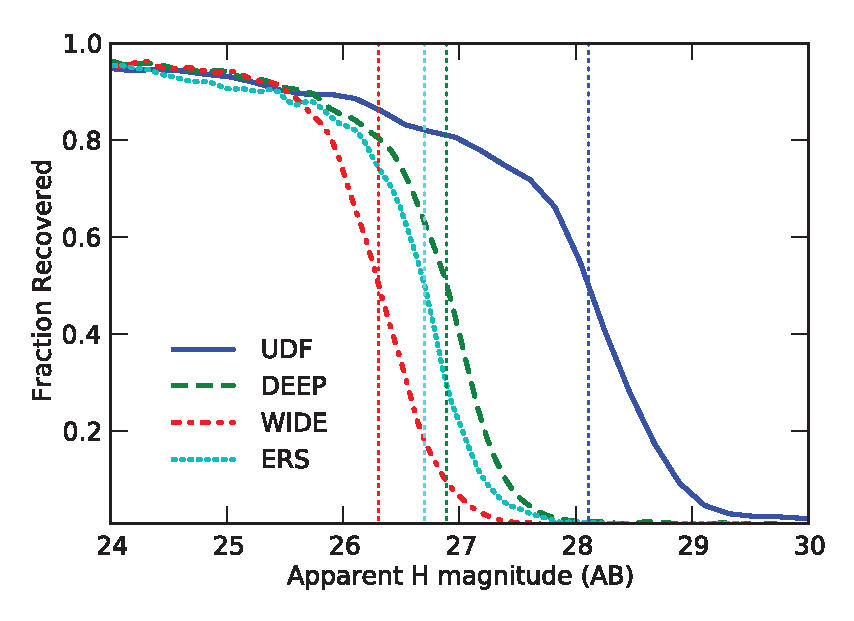
\includegraphics[width=84mm]{plots/fig3.eps}

\caption{Completeness as a function of H magnitude for each region of the GOODS South field. The vertical dashed lines show the magnitude at which the recovery fraction equals 0.5 for each region of the field.}
\label{fig:completeness}
\end{figure}

Figure~\ref{fig:completeness} shows the resulting completeness curves for each of the image regions. In \citet{Guo:2013ig}, the $H_{160}$ 50\% completeness limit is estimated using the differential number density to be 25.9, 26.6 and 28.1 for the WIDE, DEEP+ERS and UDF regions respectively. When compared to the results of a set of detection simulations similar to those undertaken in our work, \citet{Guo:2013ig} find a good agreement between the two estimations. For the UDF and DEEP+ERS regions, our 50\% completeness limits are in good agreement with those of \citet{Guo:2013ig}. However, in the WIDE region we find a 50\% completeness limit $\approx 0.5$ mag deeper for our input galaxy population.

\citet{2011A&A...532A..33G} demonstrated the significant effect that sizes and morphologies can have on the completeness simulations of high-redshift galaxies. Differences due to the distribution of sizes and slightly differing galaxy profiles used are to be expected. For all regions, the effects of confusion and blending with nearby sources results in a small fraction of input galaxies which are not recovered by the photometry, even at brighter magnitudes.

\subsection{Sample Selection}\label{sec:selection_sims}
To estimate the selection functions for each of the redshift bins, a mock photometry catalog of high-redshift galaxies was created and put through the same photometric redshift and sample selection criteria as our real sample. This catalog was constructed by first creating a sample of SEDs drawn randomly from the template sets used for fitting (both with and without nebular emission) with a distribution of $\beta$ centred at $\approx -1.8$ to $-2$, but extending out to $\beta > 1$. Redshifts were allowed to vary in the range $2.5 < z < 9$ and the templates were scaled to $\text{H}_{160}$ band magnitudes in the range $22 < \text{H}_{160} < 30$, with the corresponding magnitudes in the other filters determined by the shape of each SED.

We produced a catalog in this way, rather than using the mock photometry of semi analytic models as used in Appendix~\ref{app:selection} in order to allow the inclusion of nebular emission in subsequent tests on the stellar mass fitting and ensure good number statistics across all input magnitudes. 

In order to assign photometric errors to the mock photometry (or non-observations where appropriate), each simulated galaxy was assigned a position in the field drawn from the same set of input coordinates as used in the completeness simulations. Photometric errors were then assigned to each photometric band based on the observed flux errors of objects in the original catalog, specific to the region in which it resides (e.g. CANDELS Deep). The flux values for each SED were then perturbed by a gaussian of width equal to the photometric error.

This process does not precisely mirror the method used to produce the observed photometry as it does not include the source extraction for each band individually. However, the resulting catalog is a very good approximation with a catalog of SEDs that have realistic photometric errors and filter coverage across the field, e.g. $Y_{098}$ observations in the ERS region alone. 

To measure the selection efficiency for our high-redshift samples, 100 simulated Monte Carlo samples were created from the mock galaxy catalog using the method outlined in Section~\ref{sec:sample}. From these samples, we measured the fraction of simulated galaxies which pass the selection criteria for any of the high-redshift samples as a function of input redshift and magnitude.

\begin{figure*}
%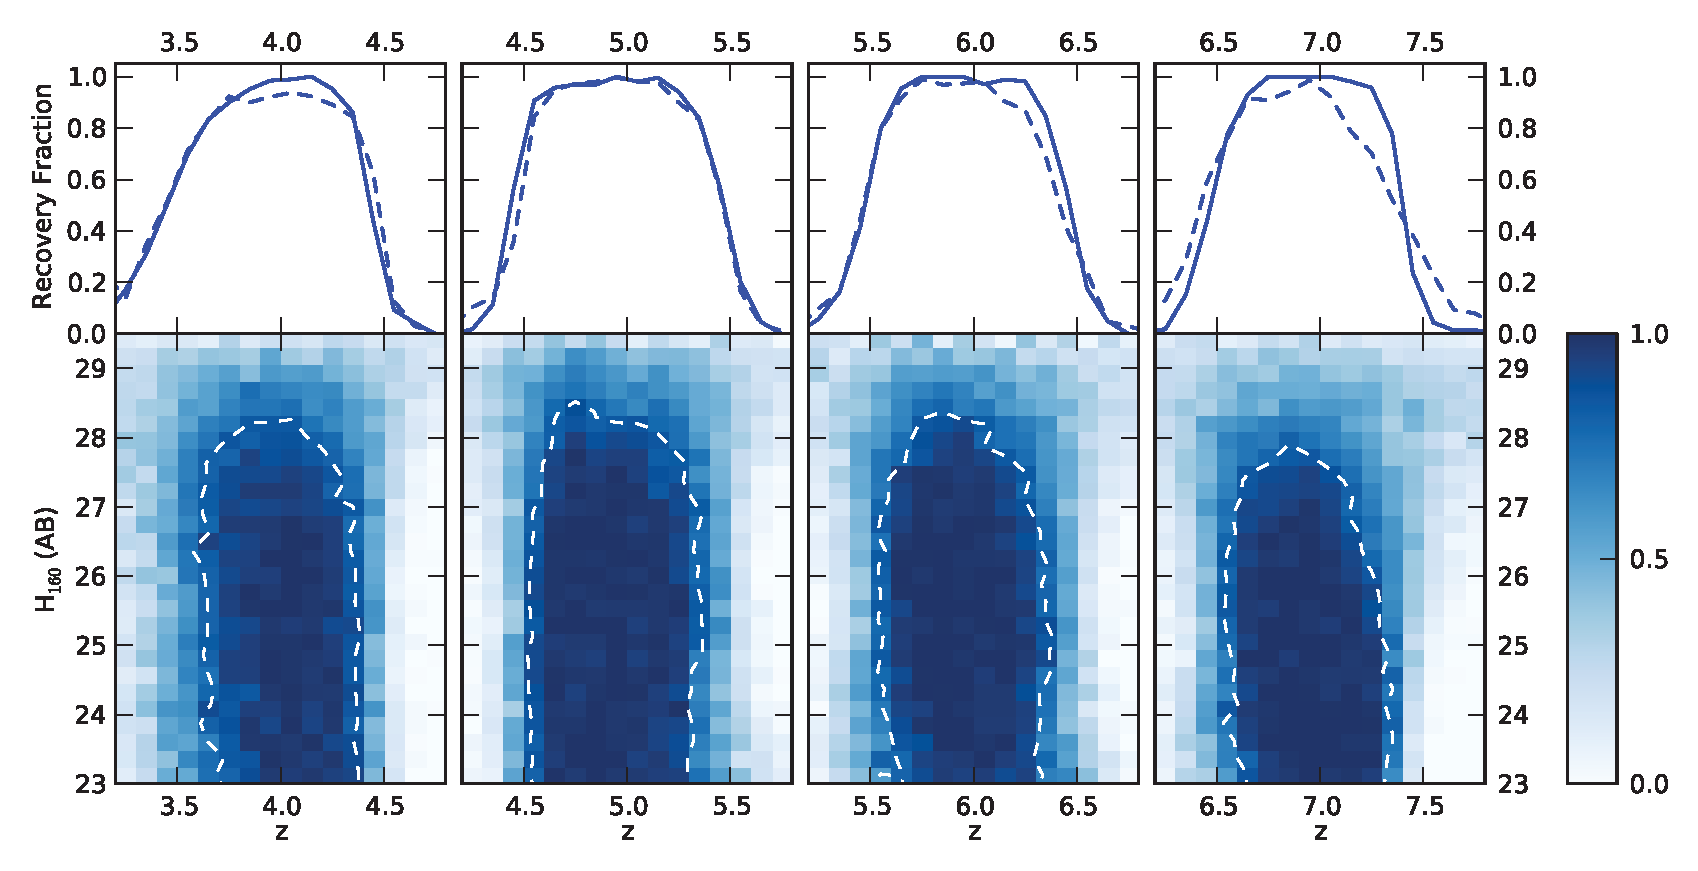
\includegraphics[width=180mm]{plots/fig4.eps}
\caption{Selection efficiencies for the Ultra Deep Field region of the CANDELS field. The colour scale represents the fraction of input galaxies which pass the $P(z)$ criteria for a given redshift bin as a function of input redshift and apparent magnitude. The dashed white line in the lower sections of the figure shows the 80\% contour in the fraction of recovered galaxies. The upper panels show the recovery fraction as a function of redshift at a fixed input magnitude, $\textup{H}_{160} = 25$ (continuous) and $\textup{H}_{160} = 27$ (dashed).}
\label{fig:selection}
\end{figure*}

Figure~\ref{fig:selection} shows the measured selection efficiencies for  the deepest region of the field, the UDF. The selection probabilities (as indicated by the colour scale) do not include the effects of completeness as measured in Section~\ref{sec:completeness}, therefore the lower probabilities measured at faint magnitude are a result of photometric redshift errors due to poor constraints from faint photometry.

For $z\sim 4$ and 5, where the semi-analytic mock catalog used in Appendix~\ref{app:selection} has good number statistics across a wide magnitude range, we reproduce the selection function in the same manner as above and find that the shape of the resulting selection functions are unchanged. We are therefore confident that the photometric selection of our samples is robust to variations in the exact shape of the input SEDs and the limiting factor in selection is the photometric noise.

\subsection{Uncertainties in measuring galaxy parameters}
The ability of SED fitting codes to recover the properties of dropout galaxies was well explored by \citet{2010ApJ...725.1644L} who found that stellar mass was the most reliably measured parameter (in comparison to star formation rate and age) and the most robust to assumptions in star-formation history. This work however was limited to SEDs excluding the effects of nebular emission only for both the input and fitted models. The degeneracies in measuring age, dust extinction and star-formation histories from SED fitting have also been well examined e.g. \citet{2010A&A...515A..73S}. It is however possible to reliably measure $\beta$ as a proxy for the stellar population properties \citep{2012ApJ...756..164F,2013MNRAS.429.2456R}.

For the $\approx 10^5$ galaxies in our simulated catalog which pass the selection criteria, we ran them through the SED fitting code using the same fitting parameters as for our observed data. From these results we are able to test how well the input stellar masses are recovered for our simulated galaxies. In addition, we can also test the accuracy in recovering the other properties of the input stellar populations.

Figure~\ref{fig:masscomparison} illustrates how well the SED code is able to recover the stellar masses, ages and dust extinction. As expected, stellar mass is the most robust of the parameters with age and dust extinction showing a very large scatter due to the degeneracy in fitting.
For input galaxies with masses $\approx 10^9 M_{\odot}$, the median(M$_{out}$-M$_{in}$) = 0.11, with a standard deviation of 0.4 when input SEDs including nebular emission are fitted with comparable templates. For input masses $\approx 10^{8.5} M_{\odot}$ and below, both the bias and scatter increase.
When mock galaxies with pure stellar SEDs are fitted with pure stellar templates, both the scatter and bias are reduced at all mass ranges. The increased bias and scatter for galaxies with nebular emission is a result of confusion between an older stellar population with a 4000\AA break and a young star-forming galaxy with strong nebular emission \citep{2009A&A...502..423S,2013MNRAS.429..302C}. Because the strength of nebular emission in the templates being fitted 

%\begin{itemize}
%\item Further Mass discussion.
%\end{itemize}

\begin{figure*}
%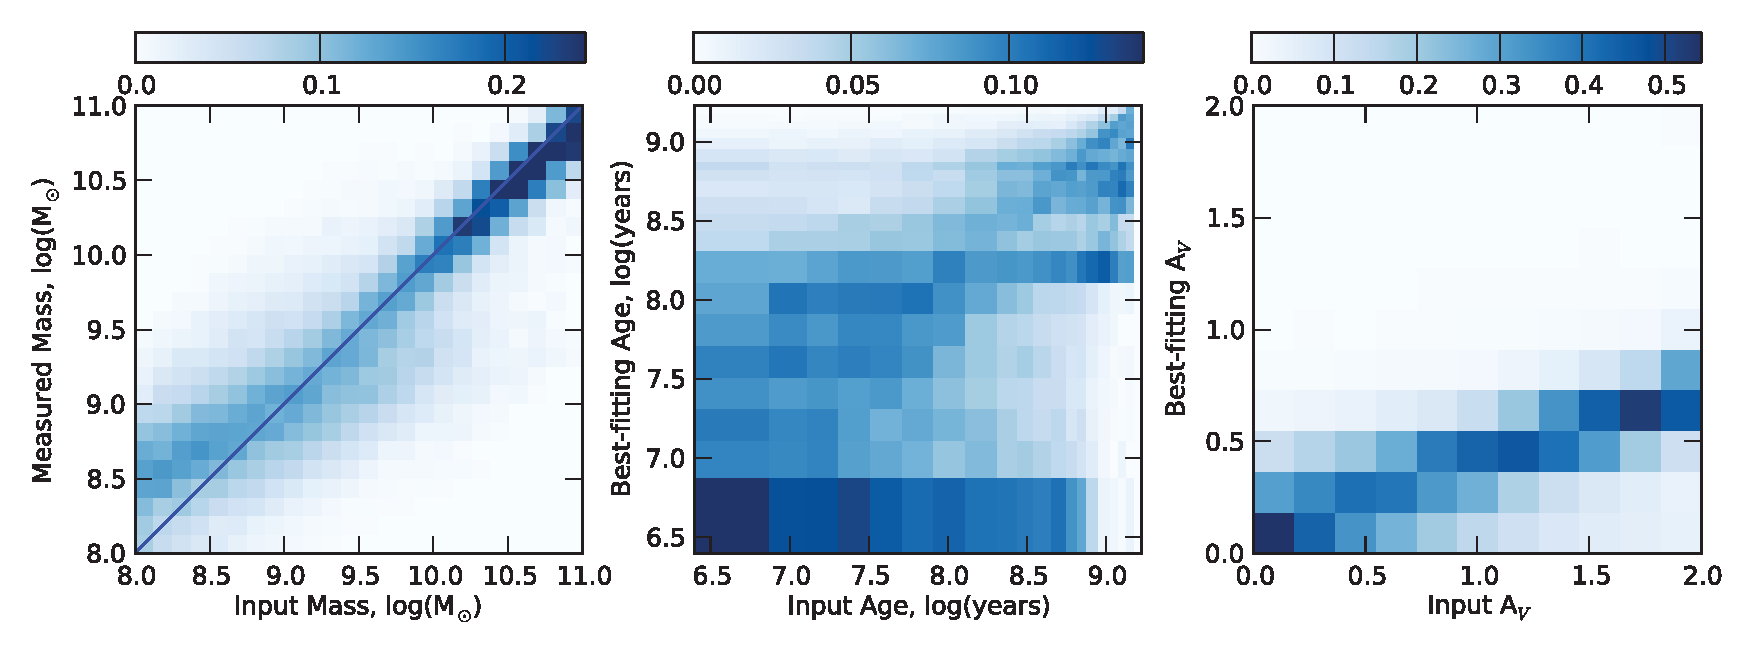
\includegraphics[width=\textwidth]{plots/fig5.eps}
\caption{2D histograms showing the recovered SED parameters for a set of input SEDs incorporating nebular emission when fitted with nebular emission. The values for the age (centre) and dust (right) are those corresponding to the single best-fitting model whilst the measured mass (left) is taken as $\int M P(M)dM$. Each histogram is normalised by the number of input galaxies in each bin and the colour scale corresponds to the fraction of input galaxies at the observed mass (/age/dust extinction) i.e. darker = more galaxies.}
\label{fig:masscomparison}
\end{figure*}

Finally, we find that the recovered value for $M_{UV,1500}$ is extremely robust across the full dynamic range of our data, with a scatter of $< 0.2$ dex and negligible bias across all redshift out to the limits of our completeness as shown in Figure~\ref{fig:muvcomparison}. From these simulations, we determine that M$_{UV,1500}$ is robust to M$_{UV} \approx$ -17 at $z \approx 4$, reducing to -18 at $z \approx 7$. The estimated accuracy of our $\beta$ measurements from these simulations is presented in Appendix~\ref{app:beta}.

\begin{figure}
%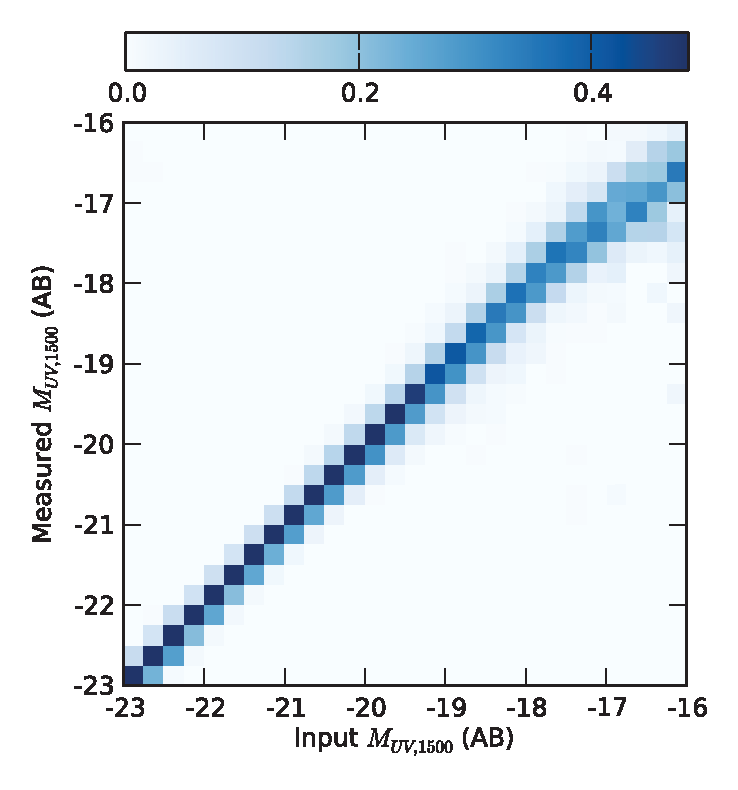
\includegraphics[width=84mm]{plots/fig6.eps}
\caption{Comparison of the recovered versus input $M_{UV}$, for the full mock galaxy sample.}
\label{fig:muvcomparison}
\end{figure}


\subsection[Subsec]{Subsection}
\label{sec:subsec1_label}

Example reference in text, \cite{ref1}.

Example reference list in text, \cite{ref1,ref2}.




%% %% End of file...  %%
